% Embedding diagram of a wormhole (Ellis throat of radius 1): the surface
%   r = sqrt(1 + l^2),  z = asinh(l),
% where l is proper radial distance through the throat. Shading is a simple
% two-sided Lambert model; the outward unit normal is
%   n = (cos(phi), sin(phi), -l) / sqrt(1 + l^2).
\documentclass[tikz,border=1pt]{standalone}
% Shared preamble for the standalone figures: the book's fonts, palette and
% drawing styles. Figures are drawn at their final printed size. A column is
% 3.35in (241pt) wide; a figure across both columns is 7in (505pt) wide.

\usepackage[T1]{fontenc}
\usepackage{newpxtext}
\usepackage[varbb]{newpxmath}
\usepackage[semibold,scale=0.95,lining]{sourcesanspro}
\usepackage{xcolor}
% Palette shared by the book and by the standalone figures in figures/src.
% One main hue (blue), one accent (orange), and a few roles used sparingly.

\definecolor{seblue}{HTML}{1D5B8F}    % headings, worked examples, main curves
\definecolor{seblueDark}{HTML}{123E63}
\definecolor{seorange}{HTML}{DC7A26}  % thought experiments, light and light cones
\definecolor{seteal}{HTML}{1F8577}    % checks, travellers and ships
\definecolor{sered}{HTML}{C0392B}     % negative energy, tension, violations
\definecolor{seviolet}{HTML}{5E548E}  % going deeper
\definecolor{sesand}{HTML}{8C6A3F}    % history
\definecolor{segray}{HTML}{6B7480}    % axes, guides, secondary labels
\definecolor{selight}{HTML}{D5DAE1}   % grids and faint rules

\usepackage{siunitx}
\usepackage{fontawesome5}
\usepackage{tikz}
\usetikzlibrary{arrows.meta,calc,positioning,decorations.pathreplacing,
  decorations.markings,shapes.geometric,fadings,shadings,patterns,3d,
  intersections,backgrounds}
\usepackage{pgfplots}
\pgfplotsset{compat=1.18}
\usepgfplotslibrary{fillbetween,groupplots,colormaps}

\tikzset{
  >={Latex[length=2.1mm,width=1.4mm]},
  every picture/.style={line cap=round, line join=round},
  lbl/.style={font=\sffamily\footnotesize, text=black!85},
  smalllbl/.style={font=\sffamily\scriptsize, text=black!75},
  guide/.style={segray, line width=0.4pt},
  axisline/.style={segray, line width=0.5pt, -{Latex[length=1.7mm,width=1.1mm]}},
  light/.style={seorange, line width=0.9pt},
  lightdash/.style={seorange, line width=0.9pt, dash pattern=on 3pt off 2pt},
  ship/.style={seteal, line width=1.4pt},
  cone/.style={fill=seorange!22, draw=seorange!85!black, line width=0.35pt},
}

\pgfplotsset{
  se axis/.style={
    axis lines=left,
    axis line style={segray, line width=0.5pt, -{Latex[length=1.6mm,width=1.1mm]}},
    tick style={segray, line width=0.4pt},
    major tick length=2.5pt,
    tick label style={font=\sffamily\scriptsize, text=black!75},
    label style={font=\sffamily\footnotesize, text=black!85},
    every axis plot/.append style={line width=1.1pt},
    legend style={font=\sffamily\scriptsize, draw=none, fill=none},
    scaled ticks=false,
    xticklabel={\sansnum{\tick}}, yticklabel={\sansnum{\tick}},
  },
}

% Numbers in figures are set in the sans-serif text font, with a true minus.
\sisetup{mode=text, reset-text-family=false, reset-text-series=false,
  reset-text-shape=false, drop-zero-decimal, group-minimum-digits=5}
% Tick values arrive as long decimals (1.5000000000); parse them first.
\newcommand{\sansnum}[1]{\begingroup\pgfkeys{/pgf/fpu=false}%
  \pgfmathparse{1*(#1)}\num{\pgfmathresult}\endgroup}

\begin{document}
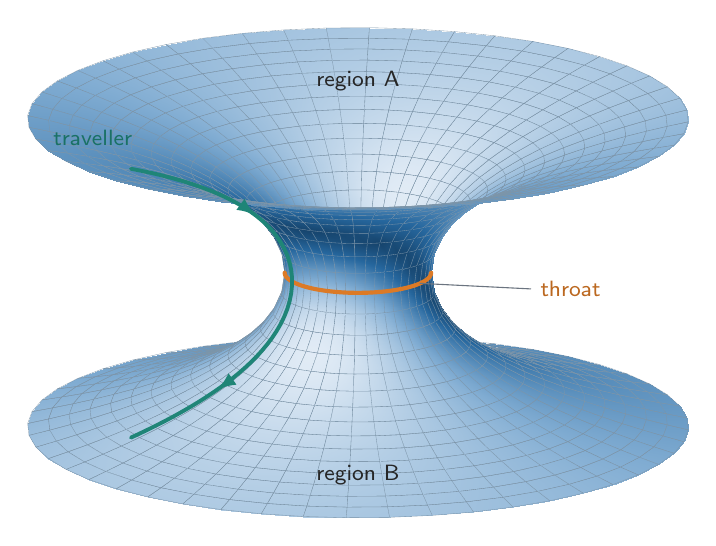
\begin{tikzpicture}
\begin{axis}[
  hide axis, view={-28}{16}, axis equal image, clip=false,
  width=368pt, height=317pt,
  colormap={worm}{rgb255(0cm)=(16,55,90) rgb255(3cm)=(38,103,158)
    rgb255(6cm)=(128,172,210) rgb255(9cm)=(226,236,246)},
  point meta min=0, point meta max=1,
]
% light from the upper left, slightly in front
\pgfmathsetmacro{\Lx}{-0.62}\pgfmathsetmacro{\Ly}{-0.42}\pgfmathsetmacro{\Lz}{0.66}
\addplot3[
  surf, shader=faceted interp, faceted color=seblueDark!55, line width=0.12pt,
  z buffer=sort, samples=31, samples y=49,
  domain=-4.4:4.4, y domain=0:360, variable=\u, variable y=\v,
  point meta={0.08 + 0.92*abs((\Lx*cos(\v) + \Ly*sin(\v) - \Lz*\u)/sqrt(1+\u^2))},
] ({sqrt(1+\u^2)*cos(\v)}, {sqrt(1+\u^2)*sin(\v)}, {ln(\u + sqrt(1+\u^2))});

% the throat: front half only (the viewer sits at azimuth 242 degrees, so the
% visible half runs from 152 to 332 degrees)
\addplot3[seorange, line width=1.5pt, domain=152:332, samples=60, samples y=1, variable=\t]
  ({cos(\t)}, {sin(\t)}, {0});

% a traveller's path through the throat, on the side facing the viewer
\addplot3[seteal, line width=1.4pt, domain=-3.3:3.3, samples=60, samples y=1, variable=\u,
  postaction={decorate}, decoration={markings,
    mark=at position 0.3 with {\arrow{Latex[length=2.4mm,width=1.8mm]}},
    mark=at position 0.78 with {\arrow{Latex[length=2.4mm,width=1.8mm]}}}]
  ({sqrt(1+\u^2)*cos(178)}, {sqrt(1+\u^2)*sin(178)}, {-ln(\u + sqrt(1+\u^2))});

\coordinate (throatlabel) at (axis cs:{cos(300)},{sin(300)},0);
\coordinate (pathstart) at (axis cs:{3.45*cos(178)},{3.45*sin(178)},1.91);
\node[lbl, anchor=south] at (axis cs:0,0,2.45) {region A};
\node[lbl, anchor=north] at (axis cs:0,0,-2.6) {region B};
\end{axis}
\draw[guide] (throatlabel) -- ++(40pt,-2pt) node[lbl, anchor=west, text=seorange!85!black] {throat};
\node[lbl, text=seteal!85!black, anchor=south east] at ($(pathstart)+(4pt,5pt)$) {traveller};
\end{tikzpicture}
\end{document}
